\chapter{Design and Implementation}
\label{designandimpl}

    \section{Introduction}
    
    In this chapter we provide an overview of the design and 
    implementation of the type analysis described in 
    section \ref{phalapproach}. Aside the type analysis 
    itself, the aim of Control Flow for Phalanger is to provide 
    a generic framework for implementation of any kind 
    of analysis, especially \emph{data-flow} based analyses.
    
    Control Flow for Phalanger includes implementation of 
    aforementioned type analysis, constant propagation analysis 
    and dead code detection. The results of those analyses 
    are made available to other user defined analyses 
    through a public interface, so that user defined analyses 
    can benefit from, for example, a resolved method call 
    that depends on the type of the variable the method 
    is called upon. Moreover, the analyses included in 
    Control Flow for Phalanger can report errors and warnings 
    discovered during analysing the code like, for instance, 
    dead code or type mismatches with documentation.
    
    Control Flow for Phalanger can also be used as a 
    library by other tools. For example, integrated 
    development environment plug-in can visualize the 
    issues reported by the default analyses, or compiler 
    can use the public interface for accessing the 
    analyses results to emit more efficient code.
    
    In the next section we discuss the implementation 
    constraints that come from the requirement to use 
    Phalanger front-end and to integrate Control Flow 
    for Phalanger with the whole Phalanger project -- 
    it should be designed so that it can be plugged 
    in between the Phalanger's front-end and back-end 
    and it should also provide public interface useful 
    for the Phalanger PHP Visual Studio tools.
    
    Section \ref{overalldesign} provides an overview 
    of the architecture of Control Flow for Phalanger in 
    terms of high level modules and their interaction. 
    Finally, the last section of this chapter \ref{impl} describes 
    some of the interesting bits of the implementation.
    
    \section{Implementation Constraints}
    
    \subsubsection*{Abstract Syntax Tree}     
    Phalanger front-end parses PHP code into an Abstract 
    Syntax Tree (AST) \cite{aho1985compilers} structure. 
    An example of such AST structure is depicted in 
    figure \ref{estexample}. This structure is then traversed 
    by the Phalanger back-end, which emits the 
    corresponding Microsoft Intermediate Language 
    (MSIL) instructions. Phalanger does not use any other 
    intermediate representation than AST and so the back-end 
    transforms AST directly to MSIL.
    
\begin{figure}[h]  
  \centering
    \includegraphics*[scale=0.5]{graphs/evaltree-ast.png}  
    \caption{Abstract Syntax Tree of code \code{(foo()+\$a)/\$b}.\label{estexample}}
\end{figure}      
    
    The classes that represent the AST nodes support extensible 
    attributes through which one can attach any additional 
    information to the nodes, or in other words, ``annotate'' the nodes. 
    This mechanism is used by Phalanger back-end and 
    Control Flow for Phalanger also uses the extensible 
    attributes to provide the results 
    of its analyses as discussed in the following section.
    
    \subsubsection*{Integrated Development Environment Integration}
    The PHP Tools for Visual Studio use Phalanger 
    front-end in order to parse PHP code into AST 
    and then the AST is again traversed to provide 
    code completion and other features. The AST nodes 
    hold necessary pieces of information, for example, 
    the position in the source file or documentation comments.
    Control Flow for Phalanger can seamlessly integrate 
    into this schema, because it provides its results 
    as annotations of the original AST nodes.
    
    The longer term aim of this project, not in the scope 
    of this \wthesis{}, is to replace the existing 
    algorithms for code completion, ``jump to definition'' 
    and ``find usages'' features. Because 
    with a dynamic language like PHP, it is not trivial to 
    find all the usages of, for example, a class or determine 
    a definition of, for instance, a field accessed 
    on some local variable. In order to provide more 
    precise results, type analysis is needed.
    
    \subsubsection*{Large PHP Projects}
    The implementation of the analysis should be able to handle 
    PHP projects with few thousands of files on a typical development 
    PC configuration under 1 minute and with less than 2GB of memory, 
    so that it can be integrated into the development process as a 
    part of a compiler or IDE plugin.
    
    \section{Overall Design}
    \label{overalldesign}
    
    The project is divided into several modules.
    \begin{itemize*}
        \item Control Flow Graph,
        \item Intermediate Representation of PHP Code (Phil, RPhil),
        \item Generic Data Flow Analysis Framework, 
        \item Tables with Type and Other Information, 
        \item Concrete Analyses:
        \begin{itemize*}
            \item Dead Code Elimination, 
            \item Aliasing Analysis, 
            \item Constant Propagation,
            \item Type Analysis.
        \end{itemize*}
    \end{itemize*}
    
    The interactions between those modules on a conceptual level 
    when performing an analysis are depicted in diagram \ref{overalldiagram}. 
    Green elements represent extension points. Red arrows represent the 
    core flow of the algorithm.

\begin{figure}[h]  
  \centering
    %\includegraphics*[width=\textwidth,height=\textheight,keepaspectratio,viewport=0 55 532 590]{img/ControlFlowModules.pdf}  
    \includegraphics*[width=\textwidth,height=\textheight,keepaspectratio,viewport=0 15 565 590]{img/ControlFlowModules.pdf}  
    \caption{Control Flow for Phalanger Design Overview\label{overalldiagram}}
\end{figure}

    In case of analysis of a single routine, the PHP source code is first 
    parsed by Phalanger front-end, then we construct a control 
    flow graph of the routine and start the Data-flow analysis. 
    Each control flow graph node, called basic block, contains AST 
    elements representing statements that are always executed 
    sequentially. The Data-flow analysis module directs the 
    generic algorithm of computing the data-flow equations, 
    but when it needs to perform a \emph{transfer function} or 
    an operation with a \emph{data-flow} value, it invokes the implementation of 
    those provided by the ``Concrete Data Flow Analysis''. 
    In order to make the implementation of \emph{transfer functions} 
    easier, the the list of basic block's AST elements is 
    transformed into an intermediate language, which is simplified 
    version of the AST elements and also includes some additional 
    information useful for analysis implementation.
    
    The analysis results can be saved as annotations of 
    corresponding AST nodes or they can be saved into the 
    \emph{global symbols} database that provides type and 
    other useful information about global symbols like 
    routines, classes, and others. Conversely, the 
    \emph{global symbols} database can be used by the 
    analysis to query the global symbols information.
    
    The following paragraphs describe some of the 
    modules in detail.

    \subsection{Intermediate Representation}
    The purpose of the intermediate representations is 
    to aid the design of the concrete analyses by 
    providing a simpler interface than full AST.
    However, at the same time, it was desirable to stay as 
    close to the original AST elements as possible in order 
    to easily propagate the results and to easily integrate 
    Control Flow for Phalanger into the Phalanger project.         
    Lastly the intermediate language should stay close enough 
    to PHP code so that PHP specific patterns can be recognized.    
    
    Control Flow for Phalanger uses two intermediate representations 
    on a conceptual level, however, they are usually not explicitly 
    constructed, but transformed from AST on the fly.
    
    \emph{Phil} stands for \emph{PHP Intermediate Language} and is 
    very abstract representations close to the original AST. 
    The main aim of Phil is to provide a framework for 
    traversing the AST elements in the order of their 
    execution in the smallest execution steps possible 
    with respect to their possible effects to the environment.     
    
    Phil contains only statements and expressions that can be 
    in a Basic Block, therefore it does not contain most of the 
    control flow changing statements like if, switch, or loops. 
    A Phil statement represents the smallest single step 
    of an execution that can change state of variables 
    or global state or throw an exception. Syntactic 
    constructs like \code{\$i++} are unfolded to 
    \code{\$i=\$i+1}, which is then split to 
    evaluation of binary expression and assignment expression 
    that uses the result of the binary expression. In some sense, 
    Phil can be viewed as a three address code.
    
    \emph{RPhil} stands for \emph{Resolved PHP Intermediate Language}. 
    RPhil is essentially Phil with resolved symbols where possible. 
    In order to resolve the symbols, the module building RPhil 
    can use names explicitly expressed in the code, for example, 
    for direct local variable access \code{\$a}, or results of 
    an analysis, for instance, results of the type analysis to 
    resolve method calls and fields references. Those results 
    are obtained from AST annotations and from \emph{global symbols}.
    RPhil itself is typically consumed by the analyses, 
    so the accuracy of RPhil and subsequently of the 
    analyses results can be improved by iterative execution 
    of the analyses.
    
    \subsection{Global Symbols}
    Global symbols database provides interface for 
    obtaining type information of global symbols, 
    namely routines, object fields, static fields, constants 
    and global variables. Definitions of those symbols can be 
    part of the analysed code or they can, for example, refer 
    to a built-in functions or external libraries. 
    For this reason, there are two interfaces 
    for the Global symbols database. 
    
    \emph{Code Tables} is a read and write interface for 
    a database of symbols that are part of the analysed code.     
    In this case the database can provide more than just type 
    information. Especially, we have a source code of definitions 
    of those symbols and so we can perform analysis in order to 
    infer their type information and save it back into 
    the \emph{Code Tables}.
    
    \emph{Type Tables} on the other hand provide only read
    access to only type information and few other important 
    pieces of information, concretely which parameters are 
    passed by reference, if a routine returns a reference 
    and similar. \emph{Type Tables} merge the data from 
    \emph{Code Tables}, which provide even more information 
    than needed, and any other user defined data source, 
    which can be, for example, a database with built-in symbols.    
        
    \subsection{Extensibility}
    The whole project is designed as a class library and 
    framework with many extension points. Some of the 
    functionality can be used independently. For example, 
    Control Flow Graph builder to generate diagrams.
    
    Nonetheless, in order to provide better usability, 
    Control Flow for Phalanger also contains 
    a simple Facade interface that plugs in together all 
    the necessary objects needed to perform a defined 
    analysis of a file or a given piece of code.
    
    \section{Implementation}
    \label{impl}
    This section describes some of the interesting parts of the 
    implementation in more detail.
    
    \subsection{Intermediate Languages Construction}
        We denote one statement of the intermediate language as
        a Phil or RPhil element. RPhil elements correspond 
        one-to-one to Phil elements, they only carry more 
        information. The aim of the implementation was to 
        save resources by not constructing the Phil (RPhil) 
        representation for every AST element explicitly and 
        saving it in memory.
        
        Under closer look, most of the AST elements correspond to 
        exactly one Phil element, or they are ignored, 
        which is the case of most control flow changing statements 
        and declaration statements. Those AST elements are used as 
        Phil elements as they are. However, elements that have to be 
        unfolded into several operations, such as \code{IncDecEx} 
        representing post or pre increment or decrement, have to 
        be represented by more elements. 
        
        One option would be to create a whole new alternative 
        AST structure that would correspond the unfolded code. 
        In our approach, we reuse the AST element to represent one 
        of the unfolded operations and create new special Phil 
        elements that wrap the original AST element and their 
        only purpose is to indicate the stage of the compound 
        operation. So for example, \code{IncDecEx} is broken down 
        to 
        \begin{itemize*}
            \item \code{Expression} that represents the variable access and 
                is recursively broken down to Phil elements, 
            \item \code{IncDecEx} that represents the binary plus operation,
            \item \code{IncDecPhilAssignment} that represents the assignment 
                and is a special additional Phil element.
        \end{itemize*}
        
        Phil elements are processed on the fly as they are transformed from 
        the original AST, therefore we do not have to explicitly save them 
        in memory. This means that every time a piece of AST is to be processed, 
        the transformation to Phil take place again, but in a fact, it is 
        a very light process. Nonetheless, we have an object instance to 
        represent every Phil element, so we do not have to process them 
        on the fly, they can also be saved into an array, which enables 
        us to perform the traversing of original AST only once, shall 
        it be a performance issue in the future.
        
        It is also possible to crate accurate control flow 
        graphs when it comes to try-catch blocks, because a single AST element, 
        can cause an exception in any stage of its evaluation, therefore it should 
        be split into single execution steps and those put into separate 
        basic blocks so that an edge from each of them to the 
        catch block can be created. Note that the design is prepared 
        for this case, but it is not implemented.
    
    \subsection{Control Flow Graph}        
        
        \subsubsection*{Exceptions}
        For try code blocks every statement is placed in 
        its own basic block that is connected to the basic block 
        of the consecutive statement and connected to all 
        the possible catch code blocks.
        
        The possible catch blocks are chosen pessimistically, so 
        a statement in try code block is connected to all the 
        catch code blocks, even nested ones, up to a catch block 
        that catches generic \code{Exception} or to the 
        graph's \emph{exit} basic block. The picture \ref{cfgthrow} show 
        a control flow graph for a function with try-catch blocks.
        
\begin{table}[h]
  \begin{tabular}{ l | m{6cm} }
  \centering
    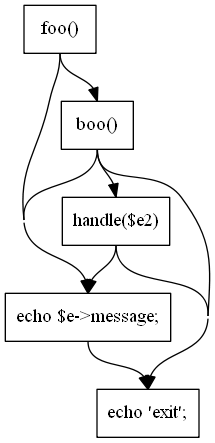
\includegraphics[scale=0.7]{src/throw.png}
  &
 
\begin{minipage}{6cm}
%pygmentize_begin php
% <?php
%    try {
%        foo();
%        try {
%            boo();
%        } catch (MyException $e2) {
%            handle($e2);
%        }
%    } catch (Exception $e) {
%        echo $e->message;
%    }
%    
%    echo 'exit';
%pygmentize_end
\end{minipage}

  \\
  \end{tabular}
  \caption{Control Flow Graph with Exceptions\label{cfgthrow}}  
\end{table}
        
        \subsubsection*{Edges}
        Control Flow Graph edges can have an optional attribute which 
        states the expression that has to hold if this edge is taken 
        during the execution. For example, an edge to then branch of 
        \code{if (\$x==3)} will have expression \code{\$x==3} and the 
        analyses may work out from it that \code{\$x} is equal to 
        \code{3} in the basic block corresponding to the then branch.
        
    \subsection{Data Flow Analysis}
        A data flow analysis (DFA) in general can be performed on any graph, 
        and so even in our case, we did not want it to be tied 
        Control Flow Graph. For this purpose, our implementation of DFA is 
        performed on interfaces that Control Flow Graph implements, 
        but they can be implemented, for example, by a definition-use 
        graph \cite{aho1985compilers} and DFA can be run on this graph too.
        The interfaces are depicted in figure \ref{graphifaces}.
        
\begin{figure}[h]  
  \centering
    \includegraphics*[width=\textwidth,height=\textheight,keepaspectratio]{img/graph-ifaces.png}  
    \caption{Generic Graph Interfaces for DFA\label{graphifaces}}
\end{figure}    

        The generic data flow framework handles the order in which the 
        graph nodes should be visited, compares the input and output 
        data flows and decides when the analysis has reached a fix-point. 
        However the concrete type of data flow, operations with data 
        flow instances and the transfer function are left to be defined 
        by a concrete analysis. In Control Flow for 
        Phalanger, two types of analysis can implemented. The basic one 
        processes only nodes; the ``branching'' one also processes edges, 
        in which case it can take the branching expressions of Control 
        Flow Graph into account, for example, but in general any information 
        that the concrete implementation of \code{IEdge} can provide.
        
        The operations with data flow objects could be carried out by the 
        objects themselves, but this would mean that already existing 
        classes that happen to be suitable for being a data flow would 
        have to be wrapped. And also one data flow representation, could 
        not have different operations for different analyses. An example 
        of this is \code{BitVector} class from .NET class library: it 
        cannot implement any additional interface, and some analysis 
        perform union of two vectors as the meet operation, while 
        others perform intersection.
        
        Nonetheless, having the data flow objects implement the operations by 
        themselves is more convenient and allows better encapsulation. 
        Because Control Flow for Phalanger is meant as a framework for as 
        well as software on its own, both scenarios are supported and 
        some convenient generics based implementations of required 
        interfaces are provided. The whole design is captured in 
        diagram \ref{dataflowifaces}.
        
\begin{figure}[h]  
  \centering
    \includegraphics*[width=\textwidth,height=\textheight,keepaspectratio]{img/dataflow-ifaces.png}  
    \caption{Interfaces for concrete Data Flow Analyses\label{dataflowifaces}}
\end{figure}

        A simple example of concrete Data Flow Analysis is the built-in 
        constant propagation analysis, which is discussed in the 
        following subsection.        
    
    \subsection{Analyses}
        \subsubsection*{Dead Code Elimination}
        
        The Dead Code Elimination is based on the Reverse Post Order 
        algorithm, which is supposed to order nodes in a way that 
        is the most beneficial for Data Flow Analysis and has to be 
        done anyway in order to perform Data Flow Analysis.
        
        Note that the Reverse Post Order algorithm as a part 
        of the Data Flow Analysis module is implemented 
        in a generic way for any \code{IGraph} implementations. 
        
        The algorithm performs a graph search from the \emph{Start} 
        node and after it finishes, the unvisited nodes are 
        at the end of the list with all the nodes. At this point, 
        the list with all the nodes is traversed from the last 
        element and the unvisited nodes are removed until a 
        first visited node is reached.
        
        The Control Flow Graph design allows to mark 
        some edges as ``not executable'' if the branching 
        condition is always false. Such edges will be ignored 
        when the Dead Code Elimination is performed, however, 
        the tagging of edges with false branching condition 
        has not been implemented in the final version.
        
        \subsubsection*{Constant Propagation}
        Constant Propagation represents a simple example of non-branched 
        implementation of a concrete Data Flow Analysis. 
        
        The lattice for the data flow values of single variable is 
        depicted in figure \ref{constlattice}. The Data Flow type is class 
        \code{ConstantPropagationDataFlow}, which wraps an array 
        that contains the value of each variable. 
        The value is an \code{object} instance, so it can be \code{null}, which 
        is the least element of the lattice, or its value can be concrete 
        singleton object instance that by convention represents 
        \code{NotAConstant}, which is the greatest element of the lattice.
        
\begin{figure}[h]  
  \centering
    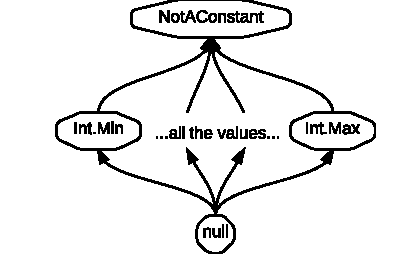
\includegraphics{img/ConstLattice.pdf}  
    \caption{The Lattice for Constant Propagation\label{constlattice}}
\end{figure}        
        
        The transfer function annotates every expression 
        with its constant value if possible. An access to a 
        variable is annotated with this variable's value 
        from the data flow, some expressions can be symbolically 
        executed using the annotations to get operands values, 
        and constants are annotated with their value retrieved 
        from Type Tables.
        
        The data flow is updated only for assignment statement, 
        reference assignment statement and for function call, 
        because some local variables can be passed by reference, 
        which can change their value. The right hand side of 
        the assignment is an expression, which should already be 
        annotated with its value that is used for the data 
        flow value.

    \subsection{Type Information Representation}        
        The theoretical side of workings of the type analysis was 
        discussed in \wsection{} \ref{phalapproach}.         
        In this paragraph we discuss representation of 
        type information for a single variable or a single expression. 
        The representation is based on the type information 
        lattice described earlier. It is a set of possible 
        basic types, class types and \code{object}. It can 
        have flags ``subclasses'' and ``type hint''. 
        There are few things to note:
        \begin{itemize*}
            \item \code{object} represents any object type, 
            \item \emph{Any} is a special \emph{data-flow} value that 
                represents any possible type, 
            \item empty set $\emptyset$  is a special \emph{data-flow} value that 
                represents uninitialized type.
        \end{itemize*}
        
        The aim is to represent the type information efficiently, 
        because we want to annotate every expression with type 
        information and because we want a memory efficient 
        representation of the \emph{data-flow}, which is an 
        array of type information for all variables.
        
        The type information is always tied to a concrete routine: 
        it is either annotation of one of the expressions in 
        the routine's body, or type of one of the local variables. 
        For every routine we create a special ``context'' object 
        with a list of all referenced types $\mathbb{T}$. This way 
        every type has a unique index. Let us denote the index 
        of type $K$ as $\mathit{index}(\mathbb{T}, K)$ the 
        type under index $i$ as $\mathit{type}(\mathbb{T}, i)$.
        Furthermore, we made an assumption that a single routine 
        is unlikely to reference more than $64$ distinct types. 
        From this follows that we can represent a subset of 
        $\mathbb{T}$ as a 64 bit integer, where bit with index 
        $i$ indicates whether the type $\mathit{type}(\mathbb{T}, i)$ 
        is present in the set or not. With this representation, 
        we can implement very efficient set operations with 
        bitwise operators.
        
        However, this representation does not reflect the 
        lattice we described earlier. We shuffle 
        the type indexes to the left and reserve first few 
        indexes from right for special bit flags:
        
        \begin{itemize*}
            \item\textbf{any flag} if present, other bits should be ignored and the whole 
                type information value is deemed as the lattice element \emph{Any}.            
            \item\textbf{object flag} if present any class types should be ignored.
            \item\textbf{type hint flag}
            \item\textbf{subclasses flag}
        \end{itemize*}
        
        From the properties of bitwise or, it follows that 
        a bitwise or (union) of two type information instances 
        represented with this schema, will give us their 
        lowest upper bound. Let us, for example, consider 
        a union of two type information instances where one 
        has \textbf{any flag} set. The union will have 
        also \textbf{any flag} set, which in the lattice 
        corresponds to $\emph{Any}\wedge{}x=\emph{Any}$ 
        for every $x$. The same behaviour works with 
        respect to the other special flags.
        
        Last thing we need to deal with is when a routine references 
        more types than the number we can represent. In such case, 
        any type whose index would be greater than $63$, is treated as 
        if its index was exactly $63$. This means that types with 
        index greater or equal to $63$ will share one bit and 
        therefore we loose precision, because we cannot distinguish those 
        types from each other. However, it is a safe approximation and 
        a price we pay for the memory efficiency.
